\subsubsection*{Apache Batik}
Apache Batik è un toolkit basato su Java per le applicazioni o applet che intendono utilizzare e manipolare immagini nel formato  Scalable Vector Graphics.
L'obiettivo del progetto Apache è fornire agli sviluppatori un insieme di moduli utilizzabili sia tutti insieme che singolarmente come supporto a specifiche soluzioni SVG. Ad esempio, nel progetto, sono stati ampiamenti utilizzati i moduli SVG Parser, SVG DOM e Trasncoder, sfruttati per analizzare i contenuti delle mappe delle aule, modificarli e trasformarli in immagini raster per la visualizzazione su dispositivi mobili.
La versione utilizzata è l'ultima, ovvero la release 1.8, che supporta completamente la versione 1.1 dello standard SVG.
\begin{figure}[!htb]
\centering%
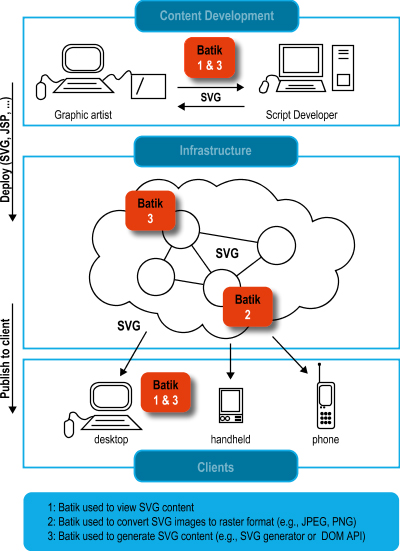
\includegraphics[scale=0.7]{batikUses.jpg}%
\caption{Esempi di utilizzo dei moduli Batik. }\label{fig:batikUsi}%
\end{figure}